\section{Avbrudd}
\label{sec:avbrudd}

\emph{Eksterne avbrytelser} refererer til situasjoner hvor en ekstern hendelse fører til en forstyrrelse i prosessen med å fullføre en oppgave \cite{Harr07}.

\subsection{Dualiteten ved avbrudd}
Grundgeiger og Sanderson (2009) \nocite{Grundgeiger09} skiller mellom \emph{gode} og \emph{dårlige} avbrudd, og hevder disse bør sees i sammenheng med hvilke effekter de har. Eksempler på positive effekter er awareness om perifer informasjon, øyeblikkelig kommunikasjon og tilgang til viktig informasjon. Avbryter opplever å få en umiddelbar bekreftelse på at informasjonen er mottatt og kan dermed avlaste arbeidsminnet, mens den som blir avbrutt kan oppleve en negativ effekt, eksempelvis at den kognitive kapasiteten overskrides, forsinkelse i eget arbeid, stress og frustrasjon. Samtidig kan avbruddet ha en positiv effekt dersom den som blir avbrutt mottar en alarm om en pasients alvorlige tilstand, eller annen ønsket informasjon.


\subsection{Avbruddshåndtering}
Gitt denne dualiteten, kan avbruddshåndtering sies å ha to mål: (1) redusere de negative effektene, og (2) utnytte de positive effektene ved avbrudd. Grandhi og Jones (2010) gir fire teknikker for avbruddshåndtering:
\begin{enumerate}        
\item Forebygging - bruk av funksjoner som forebygger eller blokkerer innkommende avbrytelser, dette gjøres ofte enkelt ved å for eksempel skru av mobilen for en periode. En annen strategi er å kontrollere timingen til avbruddet, eller å kun tillate avbrytelser som er relevant for den oppgaven man utfører. Dette krever at awareness-informasjon er tilgjengelig, slik at timingen kan justeres for å minske den negative effekten ved avbruddet.

\item Fraråding - bruk av funksjoner som fraråder avbrytelser å oppstå, dette skjer ofte ved at man gir informasjon til avbryter om tilgjengeligheten til den man ønsker å avbryte. 

\item Modifiserte varslinger - bruk av funksjoner som modifiserer hvordan individer varsles om innkommende anrop. Ved bruk av ulike modaliteter som lyd, vibrasjon og lys, kan man minimere interferensen mellom perseptuelle og kognitive prosesser involvert i avbruddshåndtering og oppgaveytelse \cite{Harr07}.

\item Forhåndsvisning - bruk av funksjoner som gir informasjon om selve avbrytelsen som den avbrutte selv kan reflektere over.   
\end{enumerate}

\noindent
\textbf{FJERNE????}
Forskere som arbeider innen \emph{interruption impact reduction}-paradigmet for avbruddshåndtering fokuserer på hvordan avbrytelser påvirker oppgaveytelse. Timing, frekvens, lengde og relevans til nåværende aktivitet eller oppgave er faktorer som påvirker de potensielle negative effektene avbruddet kan forårsake \citep{Grandhi10, Harr07}.
Målet er dermed å redusere avbruddenes negative effekt på oppgaveytelsen, og de aktuelle teknikkene for å gjøre dette er forebygging, fraråding og modifikasjon. Disse teknikkene baserer seg på den lokale konteksten til den som avbrytes. Den lokale konteksten er sammensatt av: (1) kognitiv kontekst, den kognitive eller mentale arbeidsmengden individet opplever ved gjeldende oppgave, og (2) sosial kontekst, hvor individet befinner seg og hvem som er tilstede. 
 
\noindent
Harr og Kaptelinin (2007) presenterer fler aspekter knyttet til sosial kontekst, blandt annet lokasjonsbasert forstyrrelse og indirekte forstyrrelse.

\noindent
Avbrudd kan ha effekter på andre mennesker som befinner seg på samme lokasjon som den som blir avbrutt. Dette illustreres i figur \ref{collateral}, hvor interaksjonen mellom aktør D (avbryter) og aktør B (den som avbrytes) også påvirker aktører A og C.
\begin{figure}[H]
\centering
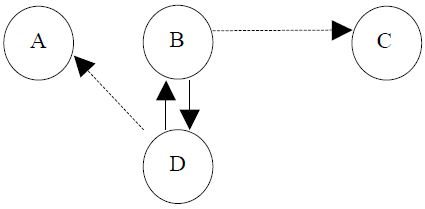
\includegraphics[scale=0.5]{collateral.jpg}
\caption{Lokasjonsbasert forstyrrelse}
\label{collateral}
\end{figure}

\noindent
Aktører B og C må ikke nødvendigvis kommunisere direkte, men aktør C kan være avhengig av tiden, innholdet og kvaliteten aktør Bs oppgave resulterer i. Dermed kan en forstyrrelse av aktør B også indirekte forstyrre aktør C.
\begin{figure}[H]
\centering
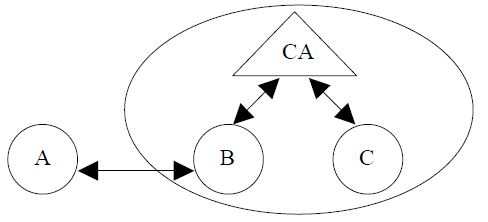
\includegraphics[scale=0.5]{dropball.jpg}
\caption{Samarbeid og avbrudd - indirekte forstyrrelse}
\label{indirekte}
\end{figure}

\noindent
\textbf{FJERNE????}
Forskere som arbeider innen \emph{interruption value evaluation}-paradigmet tar utgangspunkt i at ikke alle avbrudd er dårlige, og at de ikke bør evalueres kun avhengig av hvordan de påvirker lokal kontekst, men også avhengig av hvor stor nytte de har. Målet er dermed å optimalisere individets beslutningstakingsprosess om hvordan han skal respondere på avbruddet. Den mest aktuelle teknikken for avbruddshåndtering vil derfor være forhåndsvisning av informasjon om avbruddet, hvem det er fra og hva det handler om, slik at individet selv kan reflektere over hvordan han/hun skal respondere basert på sin lokale kontekst. Dermed vil det Grandhi og Jones (2010) kaller relasjonell kontekst være en del av avbruddskonteksten. Denne defineres som alle aspekter mellom den som avbryter og den som blir avbrutt, hvilken relasjon de har, hva avbruddet dreier seg om og deres tidligere interaksjonsmønstre, i likhet med det Harr og Kaptelinin (2007) kaller mellommenneskelige relasjoner.

\subsection{Utfordringer}
Harr og Kaptelinin (2007) påpeker tre fundamentale utfordringer ved avbruddshåndtering: (1) fare for å miste informasjon, (2) mindre privatliv og (3) utsettelse av oppgaver. For hver situasjon må individer finne den optimale balansen mellom isolasjon og tilgjengelighet, åpenhet og privatliv, og direkte eller utsatt håndtering av avbruddene.